\documentclass[twocolumn,english]{IEEEtran}
\usepackage[T1]{fontenc}
\usepackage{babel}
\usepackage{amsthm}
\usepackage{amsmath}
\usepackage{graphicx}
\usepackage[unicode=true,
 bookmarks=true,bookmarksnumbered=true,bookmarksopen=true,bookmarksopenlevel=1,
 breaklinks=false,pdfborder={0 0 0},backref=false,colorlinks=false]
 {hyperref}
\usepackage{bm}
\usepackage{amsmath}
\usepackage{amssymb}
\usepackage{natbib}
\usepackage{siunitx}
\usepackage{array}
\usepackage{calc}
\usepackage{tikz}
\newcolumntype{W}{>{\centering\arraybackslash}m{25mm}}
\newcolumntype{L}{>{\centering\arraybackslash}m{15mm}}


\hypersetup{
 pdftitle=  {Lab 4: Ohm's Law and Electrical Resistance},
 pdfauthor= {Zack Garza},
 pdfpagelayout=OneColumn, pdfnewwindow=true, pdfstartview=XYZ, plainpages=false}

\makeatletter


%%%%%%%%%%%%%%%%%%%%%%%%%%%%%% Textclass specific LaTeX commands.
 % protect \markboth against an old bug reintroduced in babel >= 3.8g
 \let\oldforeign@language\foreign@language
 \DeclareRobustCommand{\foreign@language}[1]{%
   \lowercase{\oldforeign@language{#1}}}
\theoremstyle{plain}
\newtheorem{thm}{\protect\theoremname}
\theoremstyle{plain}
\newtheorem{lem}[thm]{\protect\lemmaname}

%%%%%%%%%%%%%%%%%%%%%%%%%%%%%% User specified LaTeX commands.
% for subfigures/subtables
\ifCLASSOPTIONcompsoc
\usepackage[caption=false,font=normalsize,labelfont=sf,textfont=sf]{subfig}
\else
\usepackage[caption=false,font=footnotesize]{subfig}
\fi

\makeatother
\providecommand{\lemmaname}{Lemma}
\providecommand{\theoremname}{Theorem}
\sisetup{detect-weight=true, detect-family=true}
\setcounter{topnumber}{2}
\setcounter{bottomnumber}{2}
\setcounter{totalnumber}{4}
\renewcommand{\topfraction}{0.85}
\renewcommand{\bottomfraction}{0.85}
\renewcommand{\textfraction}{0.15}
\renewcommand{\floatpagefraction}{0.7}
\usepackage{float}
\begin{document}

\title{Ohm's Law and Electrical Resistance}


\author{Zack Garza}


\IEEEspecialpapernotice
{Physics 210L \\
Effective Date of Report: March 11, 2014 }


\markboth{Ohm's Law and Electrical Resistance}{Zack Garza}
\maketitle
\tableofcontents

\section{Introduction}
\IEEEPARstart{T}{his} experiment will investigate and important property common to all electrical circuits known as resistance. The relationship between resistance, current, and potential difference will be examined and utilized.

\noindent\textbf{Purpose}
 \begin{enumerate}
  \item To verify Ohm's Law for a simple resistive DC circuit.
  \item To calculate the resistance of an incandescent light bulb from current and voltage measurements, and to compare this to the directly measured value.
  \item To measure the current-voltage characteristics of a diode.
 \end{enumerate}



\section{Theory}

Ohm found that the ratio $R=V/I$ was nearly constant and\textbf{ nearly independent of the applied voltage $V$} for many materials. This fact is now called\textbf{ Ohm's Law}, and is predicted by theory. Note that Ohm's Law is \textit{not} $R=VI$ as is often claimed. This is the \textbf{definition of resistance} and is true for all materials. Ohm's Law, on the other hand, makes a strong claim that this ratio is \textbf{constant and independent of $V$} for many (but not all) materials, at least over a limited range of applied current.

\textbf{Part 1} measures a resistor that behaves linearly and thus obeys Ohm's Law. \textbf{Part 2} uses an identical setup to investigate a resistive element whose resistance changes as a function of applied voltage and temperature. \textbf{Part 3} examines the $IV$ characteristics of a diode by varying the voltage across it and measuring the current through it.

\section{Methodology}

\subsection*{Part 1}

\begin{enumerate}
 \item The resistance of a known resistor was measured with a DMM and recorded, as was the resistance given by its color code.
 \item The included circuit was constructed using the known resistor as $R$.
 \item The maximum possible current was calculated to be no more than $150 mA$ at the highest possible voltage delivered by the power source, and it was determined that it was safe to set the ammeter to the $430 mA$ mode.
 \item The power supply was set to a minimum output, and the circuit was activated. 10 ordered pairs for ($V,i$) were collected for the resistor $R$ over the power supply's voltage range.
\end{enumerate}

\subsection*{Part 2}

\begin{enumerate}
 \item The circuit shown in \textbf{Part 1} was rewired to a $60 V$ power supply, using a light bulb as the resistor $R$.
 \item The resistance of the light bulb was measured and recorded.
 \item The current was slowly increased to find the maximum voltage supplied by the power supply, and then reset to zero volts.
 \item Starting from the lowest voltage reading, ordered pairs ($V,i$) were collected over an approximately $60 V$ range.
 \item The resistance of the heated light bulb was disconnected from the circuit and again measured and recorded.
\end{enumerate}

\subsection*{Part 3}
\begin{enumerate}
 \item The circuit shown was wired to a $12 V$ power supply.
 \item With the potentiometer set to the fully counter-clockwise position, ordered pairs for ($V,i$) were collected as the potentiometer was slowly rotated clockwise. Extra data points were taken over particularly nonlinear regions.
 \item The leads from the power supply were reversed, and the voltage was varied in order to obtain values for the diode's reverse current and potential difference.
\end{enumerate}
\newpage
\section{Data}
\subsection*{\textbf{Part 1}}
  \begin{table}[H]
  \caption{Voltage and Current Through Known Resistor}
  \centering{}
  \label{tb:data_part1}
  \begin{tabular}{|c|c|c|}
  \hline
  \textbf{Trial} & \textbf{Voltage (V)} & \textbf{Current (mA)} \\ \hline
  1              & 2.347                & 11.7                  \\ \hline
  2              & 2.400                & 12.0                  \\ \hline
  3              & 3.824                & 19.1                  \\ \hline
  4              & 6.82                 & 34.0                  \\ \hline
  5              & 8.53                 & 42.6                  \\ \hline
  6              & 11.19                & 55.8                  \\ \hline
  7              & 13.36                & 66.7                  \\ \hline
  8              & 16.89                & 84.2                  \\ \hline
  9              & 21.29                & 106.1                 \\ \hline
  10             & 22.92                & 114.2                 \\ \hline
  \end{tabular}
  \end{table}
  \begin{align*}
  &\text{Measured Resistance (Before Trials):} 		&\text{\underline{200.7$\Omega$} } 	\\
  &\text{Measured Resistance (After Trials):} 		&\text{\underline{198.6$\Omega$} }	\\
  &\text{Color Code Resistance:}			&\text{\underline{201$\Omega$} }	\\
  \end{align*}
\subsection*{\textbf{Part 2}}
  \begin{table}[H]
  \caption{Voltage and Current Through Incandescent Light Bulb}
  \centering{}
  \label{tb:data_part2}
  \begin{tabular}{|c|c|c|}
  \hline
  \textbf{Trial} & \textbf{Voltage (V)} & \textbf{Current (mA)} \\ \hline
  1              & 2.031                & 17.2                  \\ \hline
  2              & 4.56                 & 27.5                  \\ \hline
  3              & 6.56                 & 34.1                  \\ \hline
  4              & 9.31                 & 41.9                  \\ \hline
  5              & 12.81                & 50.7                  \\ \hline
  6              & 16.51                & 58.9                  \\ \hline
  7              & 20.78                & 68.2                  \\ \hline
  8              & 25.96                & 77.6                  \\ \hline
  9              & 29.78                & 84.4                  \\ \hline
  10             & 34.19                & 91.7                  \\ \hline
  11             & 38.38                & 98.3                  \\ \hline
  12             & 43.2                 & 105.5                 \\ \hline
  13             & 48.7                 & 113.3                 \\ \hline
  14             & 53.8                 & 120.4                 \\ \hline
  15             & 58.5                 & 126.6                 \\ \hline
  \end{tabular}
  \end{table}
  \begin{align*}
  &\text{Measured Resistance (Before Trials):} 		&\text{\underline{48.2$\Omega$} } 	\\
  &\text{Measured Resistance (After Trials):} 		&\text{\underline{64.3$\Omega$} }	\\
  \end{align*}
\subsection*{\textbf{Part 3}}
  \begin{table}[H]
  \caption{Voltage and Current Measurements of Diode}
  \centering{}
  \label{tb:data_part3a}
  \begin{tabular}{|c|c|c|}
  \hline
  \textbf{Trial} & \textbf{Voltage (V)} & \textbf{Current (mA)} \\ \hline
  1              & 0.725                & 29.6                  \\ \hline
  2              & 0.724                & 29.0                  \\ \hline
  3              & 0.723                & 28.7                  \\ \hline
  4              & 0.722                & 28.0                  \\ \hline
  5              & 0.721                & 27.6                  \\ \hline
  6              & 0.720                & 27.1                  \\ \hline
  7              & 0.719                & 26.1                  \\ \hline
  8              & 0.718                & 25.5                  \\ \hline
  9              & 0.717                & 25.1                  \\ \hline
  10             & 0.716                & 24.5                  \\ \hline
  11             & 0.715                & 23.6                  \\ \hline
  12             & 0.714                & 23.2                  \\ \hline
  13             & 0.712                & 22.3                  \\ \hline
  14             & 0.710                & 21.5                  \\ \hline
  15             & 0.708                & 20.6                  \\ \hline
  16             & 0.705                & 19.2                  \\ \hline
  17             & 0.702                & 18.2                  \\ \hline
  18             & 0.700                & 17.3                  \\ \hline
  19             & 0.698                & 16.7                  \\ \hline
  20             & 0.696                & 16.1                  \\ \hline
  21             & 0.695                & 16.0                  \\ \hline
  22             & 0.693                & 15.0                  \\ \hline
  23             & 0.692                & 15.2                  \\ \hline
  24             & 0.690                & 14.3                  \\ \hline
  25             & 0.687                & 13.5                  \\ \hline
  26             & 0.685                & 12.9                  \\ \hline
  27             & 0.682                & 12.2                  \\ \hline
  28             & 0.680                & 11.6                  \\ \hline
  29             & 0.678                & 11.1                  \\ \hline
  30             & 0.675                & 10.6                  \\ \hline
  31             & 0.673                & 10.0                  \\ \hline
  32             & 0.670                & 9.5                   \\ \hline
  33             & 0.667                & 9.6                   \\ \hline
  34             & 0.665                & 8.4                   \\ \hline
  35             & 0.663                & 8.1                   \\ \hline
  \end{tabular}
  \end{table}
  \begin{table}[H]
  \caption{Diode Circuit Measurements with Reversed Voltage}
  \centering{}
  \label{tb:data_part3b}
  \begin{tabular}{|c|c|c|}
  \hline
  \textbf{Trial} & \textbf{Voltage (V)} & \textbf{Current ($\mu$A)} \\ \hline
  1              & -1.467               & -0.1                      \\ \hline
  2              & -2.167               & -0.2                      \\ \hline
  3              & -3.165               & -0.3                      \\ \hline
  4              & -4.51                & -0.4                      \\ \hline
  5              & -5.09                & -0.5                      \\ \hline
  6              & -6.18                & -0.6                      \\ \hline
  7              & -7.24                & -0.7                      \\ \hline
  8              & -8.12                & -0.8                      \\ \hline
  9              & -9.37                & -0.9                      \\ \hline
  10             & -10.67               & -1                        \\ \hline
  11             & -12.07               & -1.1                      \\ \hline
  12             & -13.57               & -1.3                      \\ \hline
  \end{tabular}
  \end{table}
  \begin{align*}
  &\text{Applied Voltage:} 		&\text{\underline{11.97 V} } 	\\
  &\text{Room Temperature:} 		&\text{\underline{\SI{22.5}{\degreeCelsius}}}
  \end{align*}

\section{Analysis, Results, and Conclusions}
\subsection*{Part 1}
  \begin{figure}[H]
  \begin{centering}
  \begin{center}
  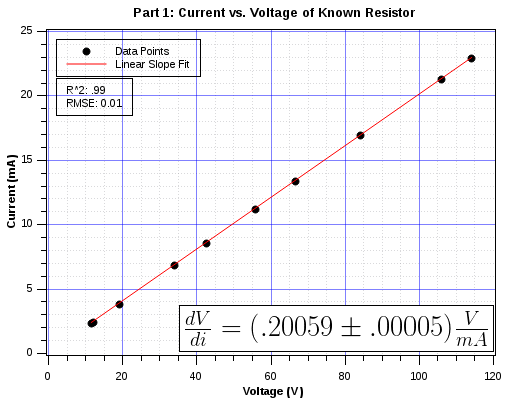
\includegraphics[width=\linewidth]{./Pictures/part1graph.png}
  \caption{Plot and Linear Fit of Table~\ref{tb:data_part1} Data.}
  \label{fig:graph_part1}
  \end{center}
  \par\end{centering}
  \end{figure}

  \begin{align*}
  &\text{Measured $R$ (Before Trials):} 			&\text{\underline{200.7$\Omega$} } 	\\
  &\text{Measured $R$ (After Trials):} 				&\text{\underline{198.6$\Omega$} }	\\
  &\text{Percent Change (Before/After):}			&\text{\underline{-1.0\%} }		\\ \\
  &\text{Measured $R_{\text{avg}}$ (Before/After):}		&\text{\underline{199.7$\Omega$} }	\\
  &\text{Color Code $R$:}					&\text{\underline{201$\Omega$} }	\\
  &\text{Percent Difference (Color/$R_{\text{avg}}$ ):}		&\text{\underline{-0.65\%} }		\\ \\
  &\text{$R$ From Linear Fit:}					&\text{\underline{(200.59 $\pm$.05)$\Omega$} }	\\
  &\text{Percent Difference (Fit/$R_{\text{avg}}$):}		&\text{\underline{0.45\%} }		\\ \\
  \end{align*}
  It was found that the measured value of $R$ changed slightly over the course of this portion of the experiment, so two measurements were taken -- one before running the trials, and one afterwards. As the resistor heated up, the resistance dropped, and so the average value of these two measurements was used as the measured value of $R$. In light of the results, the linear fit of current vs. voltage yielded a slightly more accurate value of the resistance $R$, despite the variance of the resistance while the measurements were taking place.

\noindent\hrulefill
\subsection*{Part 2}
  \begin{figure}[H]
  \begin{centering}
  \begin{center}
  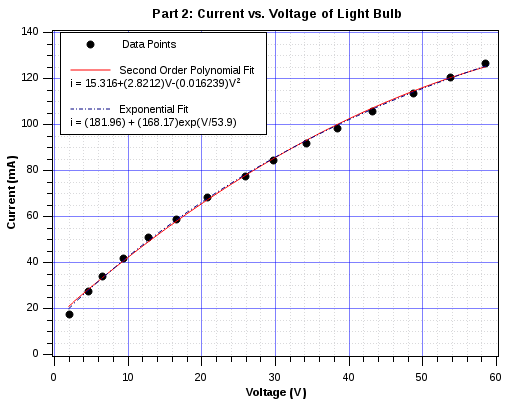
\includegraphics[width=\linewidth]{./Pictures/part2graph.png}
  \caption{Plot and Various Fits of Light Bulb Voltage and Current}
  \label{fig:graph_part2}
  \end{center}
  \par\end{centering}
  \end{figure}
  \begin{align*}
  &\text{Measured $R_{\text{Bulb}}$ (Before Trials):} 		&\text{\underline{48.2$\Omega$} } 	\\
  &\text{Measured $R_{\text{Bulb}}$ (After Trials):} 		&\text{\underline{64.3$\Omega$} }	\\
  &\text{Average $R_{\text{Bulb}}$ (Before/After):}		&\text{\underline{56.25$\Omega$} }	\\
  \end{align*}
  The plotted data shows that the incandescent light bulb departed significantly from the linear relationship $R=i/V$. Line fits were attempted with polynomial and exponential functions, but neither yielded any information that correlated with any physical measurements that were taken. This indicates that the coefficients found may be dependent on a property that was not investigated in this experiment, or that the function that governs the resistive behavior of the bulb is more complicated than the functions used. It is possible that in non-ohmic materials, the resistance could a function of other variables, such as temperature or the rate of power dissipation. Further investigations might include performing similar plots for a wider variety of such materials, and searching for common elements among the resulting functions.

\noindent\hrulefill
\subsection*{Part 3}
  \begin{figure}[H]
  \begin{centering}
  \begin{center}
  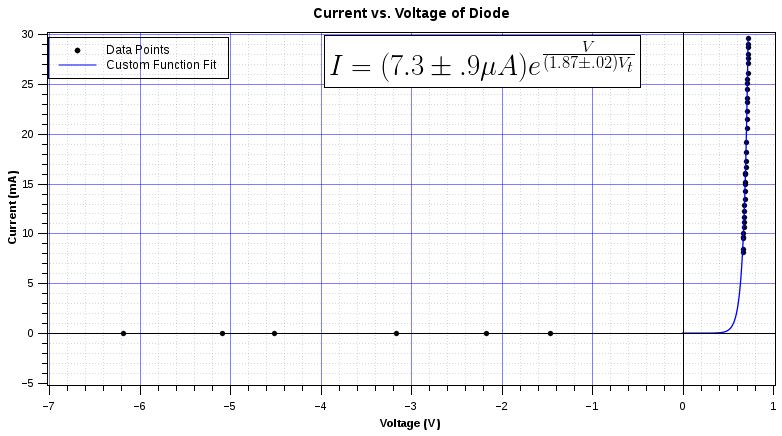
\includegraphics[width=\linewidth]{./Pictures/part3graph.png}
  \caption{Plot and Custom Fit of Diode Forward and Reverse Voltage/Current}
  \label{fig:graph_part3}
  \end{center}
  \par\end{centering}
  \end{figure}
\appendices{}
  \begin{align*}
  &\text{$n$ (From Graph):} 					&\text{\underline{$1.87\pm.02$} } 	\\
  &\text{$I_s$ (From Graph):} 					&\text{\underline{$(7.3 \pm .9) \mu A$} }	\\
  \end{align*}
  The diode's measurements were plotted and fitted according to the equation
  \begin{equation}
   i = I_s\left(e^{\frac{V}{nV_t}}-1\right)
  \end{equation}
  where $V_T$ was set equal to the constant $kT/e$, while $n$ and $I_s$ were used as fitting parameters. It was expected that the experiment would yield a value for $n$ between 1 and 2, and the results indicated that this was indeed the case. It was also expected that the saturation current would be relatively low, and the fit yielded a value of $I_s$ in the $\mu A$ range. From the data obtained for the negative voltage, however, it is clear that the current that runs backwards through the diode, while approximately 1000 times smaller than the current flowing through in forward-bias, is still non-zero and increases in proportion to applied voltage. Further experiments to test this behavior might involve increasing the reverse voltage to observe the continuation of the graph's behavior.


%\bibliographystyle{plain}
%\bibliography{physbib}

\end{document}